\section{Planar Graphs}
\frame{

\frametitle{\secname}
\begin{columns}
\column{0.6\textwidth}
\begin{wideitemize}
\item<1-> Deleting vertices or contracting/deleting edges can't turn a planar graph into a non-planar graph.

\item<2-> \textbf{Wagner's Theorem}: 

A graph is planar if and only if you cannot form a $K_5$ or $K_{3,3}$ using deletions and contractions.

\item<2-> $K_5$ are $K_{3,3}$ the \textbf{forbidden graph minors} of the family of planar graphs.
\end{wideitemize}
\column{0.05\textwidth}

\column{0.35\textwidth}
\only<1>
{
\centering
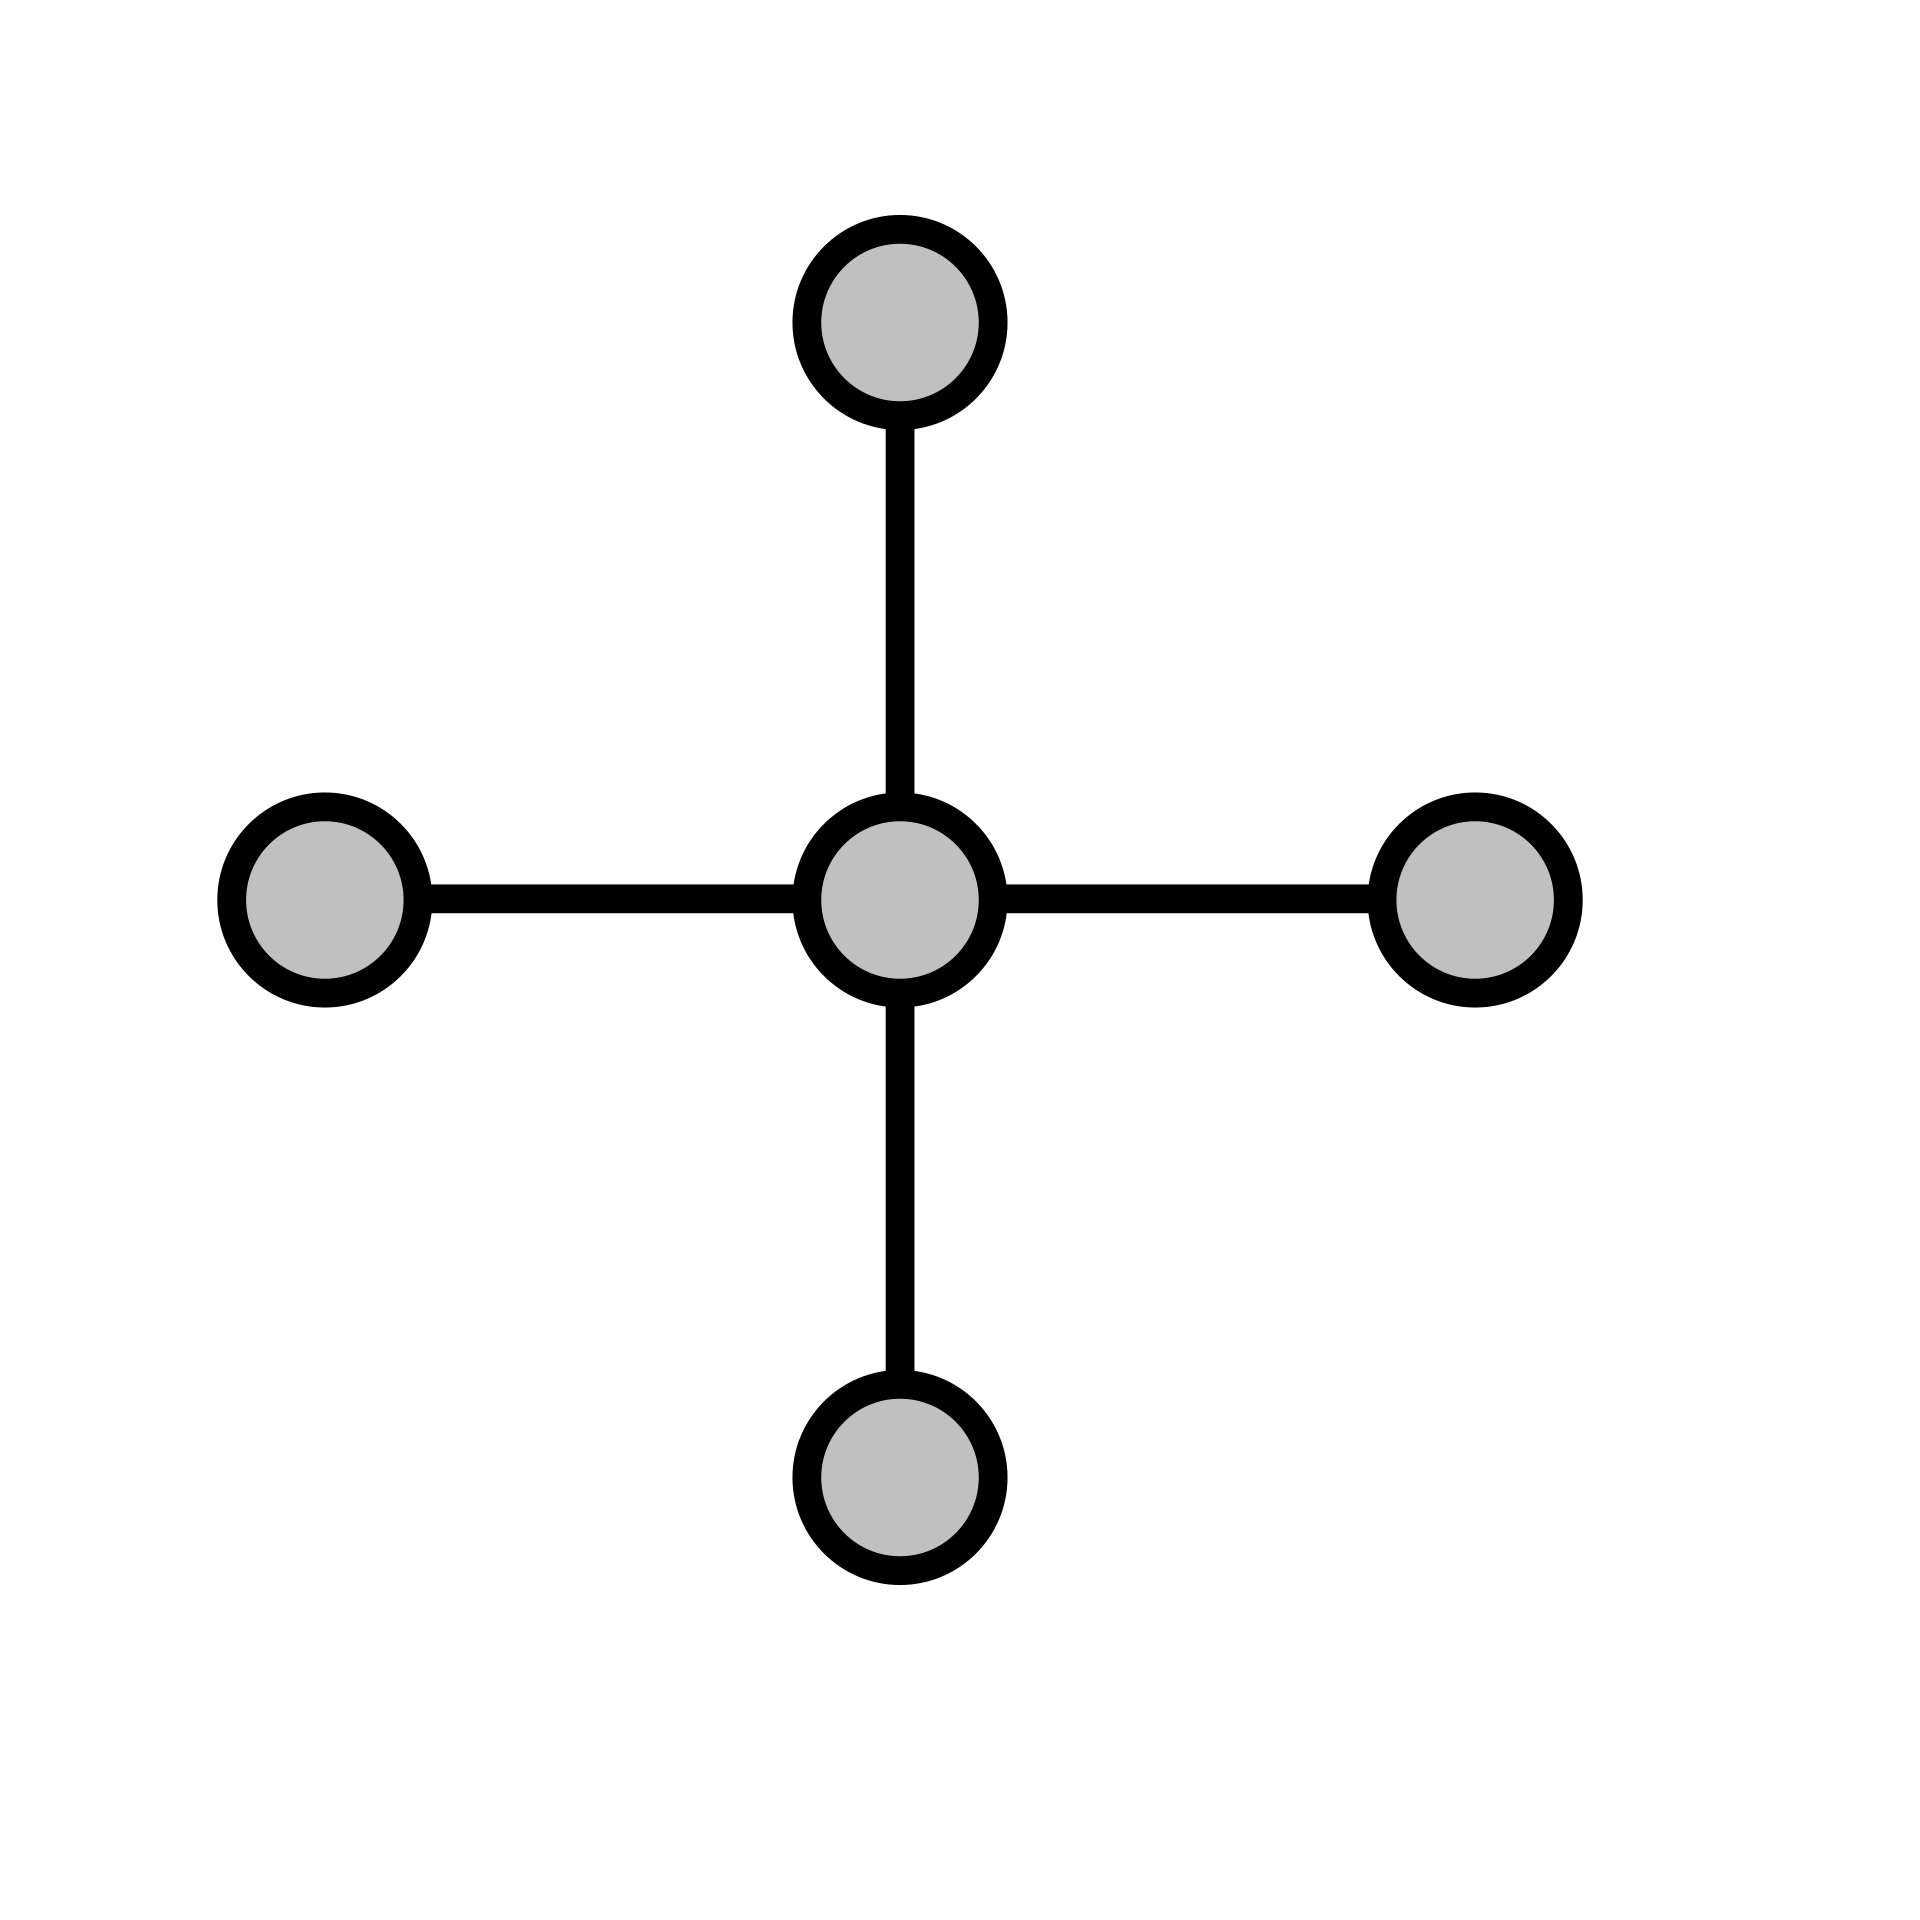
\includegraphics[width=0.3\linewidth]{slides//forbidden_minors/forbidden_minor_H.png}
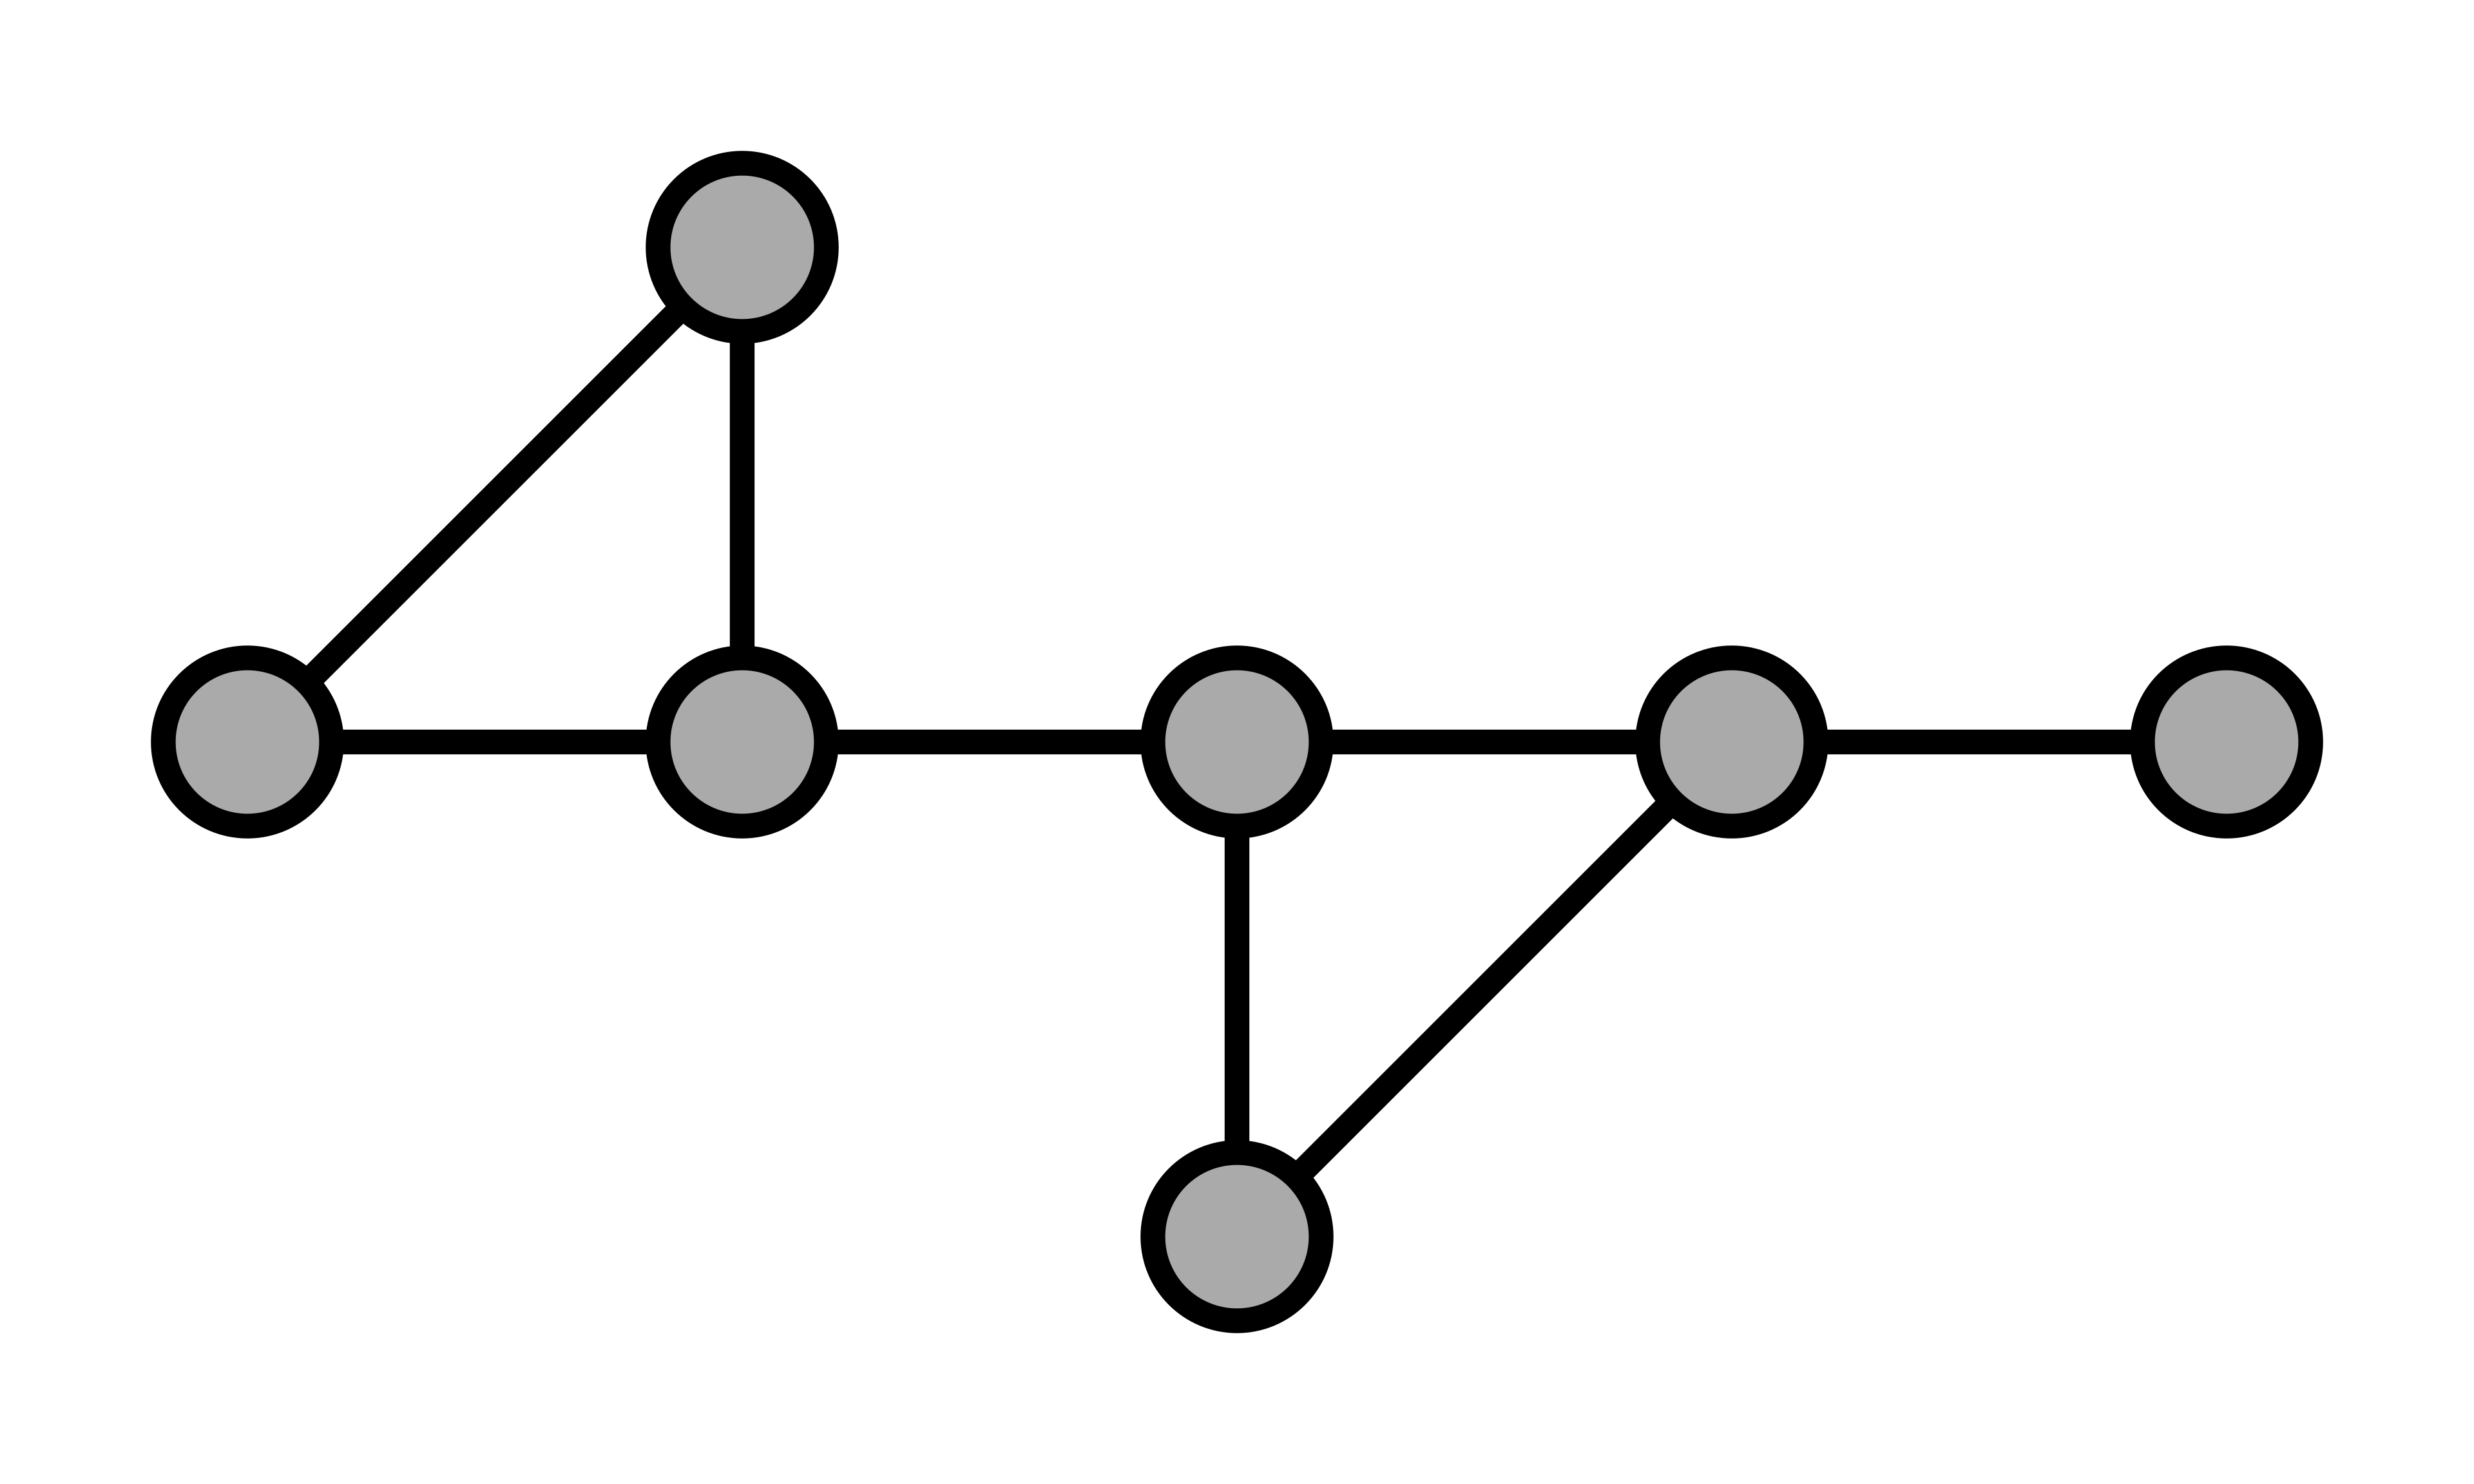
\includegraphics[width=0.5\linewidth]{slides//forbidden_minors/forbidden_minor_G.png}
\begin{figure}
    \centering
    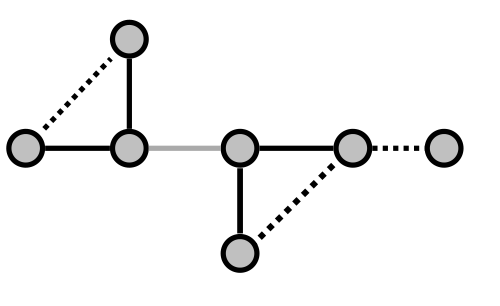
\includegraphics[width=0.6\linewidth]{slides//forbidden_minors/forbidden_minor_contraction.png}
\end{figure}
{ \tiny  diagrams from \href{https://en.wikipedia.org/wiki/Graph\_minor}{Wikimedia} }
}

\only<2->
{
\centering
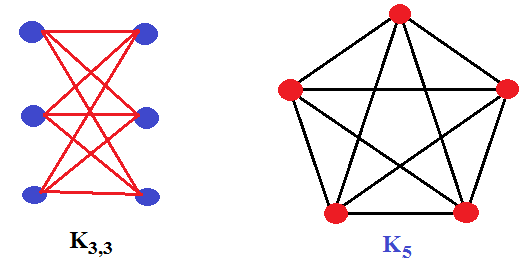
\includegraphics[width=\linewidth]{slides//forbidden_minors/forbidden_minors_k33k5.png}
{ \tiny diagrams from \href{https://upload.wikimedia.org/wikipedia/commons/4/40/K3\%2C3\_v\%C3\%A0\_K5.png}{Wikimedia} }
}

\end{columns}

}


\section{Forbidden Minors}
\frame{

\frametitle{\secname}
\begin{columns}
\column{0.8\textwidth}
\begin{wideitemize}
\item $H$ is a \textbf{graph minor} of $G$ if $H$ can be obtained from $G$ by deleting edges, isolated vertices \textbf{or} contracting edges.


\item A family $\mathcal{F}$ of graphs is \textbf{closed under taking minors} if every minor of a graph in $\mathcal{F}$ also belongs to $\mathcal{F}$.



\item \textbf{Robertson–Seymour theorem}: 

Every family of graphs that is closed under taking minors can be defined by a finite set of forbidden minors.
\end{wideitemize}

\column{0.2\textwidth}


\end{columns}

}
